% IEEE conference paper — compile with pdflatex (IEEEtran required).
% Source of truth: reports/paper/paper_content.py
\documentclass[conference]{IEEEtran}
\usepackage[utf8]{inputenc}
\usepackage[T1]{fontenc}
\usepackage{graphicx}
\usepackage{booktabs}
\usepackage{amsmath}
\usepackage{array}
\usepackage{url}
\hyphenpenalty=1000
\begin{document}
\title{Predicting District-Level Prevalence of Dilapidated Census Houses in India Using Machine Learning}
\author{\IEEEauthorblockN{Samrud}
\IEEEauthorblockA{Department of Computer Science and Engineering \\ Institution, India}}
\maketitle

\begin{abstract}
Housing condition is a direct, census-measurable dimension of deprivation, yet district-level predictive benchmarks for it are scarce. This paper predicts the prevalence of dilapidated census houses across Indian districts from Census 2011 socioeconomic and housing-stock indicators. The target is the Census-computed share of a district's census houses classified as Dilapidated; an earlier formulation using a household denominator was rejected after the denominator was shown to represent the census-house stock (330.8 million) rather than households (246.7 million). Two feature configurations were compared: a full-coverage configuration (640 districts, 43 predictors) and an expanded configuration adding household-normalised housing variables (628 districts, 77 predictors). Ten model families were evaluated under five-fold nested cross-validation grouped by state, so that reported error reflects transfer to unseen states. Under this protocol the expanded configuration improved eight of ten families, and support vector regression with an RBF kernel achieved the lowest mean absolute error (MAE 1.7248 percentage points, $R^2$ 0.3992, Spearman 0.6258); Ridge regression ($\alpha$ = 100) was retained as the primary interpretable model at MAE 1.7490. Random cross-validation understated error by 0.58-0.75 percentage points. Error analysis exposed systematic under-prediction of the most deprived districts: the 35 districts above the 95th percentile were under-predicted by 4.510 percentage points although the model was nearly unbiased overall (+0.092). Five pre-registered remedies reduced this tail bias by 18-34\% but raised overall MAE by 9.4-66.4\%; none satisfied the registered acceptance criteria and none was promoted. The results quantify the cost of honest geographic validation and the difficulty of correcting tail error with the available predictors.
\end{abstract}

\begin{IEEEkeywords}
Machine learning, housing deprivation, census data, district-level prediction, geographic generalisation, regression, grouped cross-validation, quantile regression, India.
\end{IEEEkeywords}

\section{Introduction}

The physical condition of a dwelling is among the most directly observable dimensions of deprivation, and it is the dimension on which national statistical systems most often collect comparable data. In India the decennial census classifies every census house as Good, Livable or Dilapidated, giving a prevalence measure that is defined identically across the country and reported for every district [1], [2]. Approximately 5\% of Indian census houses were classified as dilapidated in 2011, but the district-level distribution is strongly right-skewed: the median district is close to 4.4\% while the upper tail exceeds 17\%.

That skew matters for policy and for modelling. Districts in the upper tail are precisely those for which an early-warning signal would be most valuable, and precisely those that a variance-reducing estimator predicts least accurately. A regression model optimised for mean error will compress predictions toward the centre and systematically understate conditions in the districts of greatest concern.

A second difficulty is validation. Districts are nested within states, and districts of the same state share administration, climate, construction practice and reporting conventions. Random k-fold splitting therefore places near-duplicate contexts on both sides of the split and yields optimistic error estimates. Grouping folds by state converts the evaluation into a test of transfer to unseen administrative contexts, which is the operationally relevant question but a considerably harder one.

This paper reports a predictive study of district-level dilapidated-house prevalence using Census 2011 data, ten model families, nested state-grouped cross-validation, and a pre-registered investigation of tail-aware remedies. The study is observational, cross-sectional and ecological: it predicts district aggregates and makes no claim about individual households, about homelessness, about causality, or about present-day conditions.

The contributions are: (i) construction of a district-level prediction dataset by harmonising four Census 2011 sources; (ii) validation of the target definition and rejection of an incorrect denominator; (iii) an empirical comparison of a full-coverage and an expanded feature configuration; (iv) evaluation of ten model families under nested state-grouped cross-validation; (v) quantification of the gap between random and geographically grouped validation; (vi) error and interpretability analysis identifying systematic tail under-prediction; and (vii) a controlled, pre-registered test of tail weighting and quantile regression that is reported as a negative result.

\section{Related Work}

Housing deprivation is conventionally measured through dwelling condition, access to services and crowding. International monitoring frameworks treat insecure or inadequate dwelling structure as a core deprivation indicator [3], and the Indian census operationalises condition through an enumerator classification of the census house [1]. Because the classification is applied uniformly, the resulting district prevalence is comparable across regions in a way that survey-based deprivation indices often are not.

Predictive work on socioeconomic outcomes from census and administrative data has largely favoured regularised linear models and tree ensembles. Ridge regression stabilises coefficient estimates under collinearity by penalising their squared magnitude [4]; the lasso performs selection through an L1 penalty [5], and the elastic net interpolates between the two [6]. Tree ensembles aggregate decorrelated learners [7], [8], [9], while kernel methods such as support vector regression fit margin-based non-linear functions [10], and nearest-neighbour rules provide a non-parametric reference [11]. When predictors are compositional shares measured on a common base, collinearity is structural rather than incidental, which favours penalised estimation.

Validation design has received less attention than model choice in applied work, although its effect on reported performance is often larger. Roberts et al. [12] set out cross-validation strategies for clustered, hierarchical and spatial data, and Ploton et al. [13] showed that non-spatial validation can report substantial explanatory power for models whose spatial predictive power is close to null. The present study treats state grouping as a minimum requirement rather than an optional refinement, and reports the random-split result only as a reference.

Right-skewed outcomes motivate estimation of conditional quantiles rather than conditional means. Quantile regression minimises an asymmetric absolute loss [14] and is the natural tool when under-prediction of an upper tail is the failure of interest; its calibration is assessed by empirical coverage with binomial uncertainty [15], [16]. Interpretability of fitted models is commonly addressed through permutation importance [7] and through the stability of coefficients across resamples.

What remains insufficiently investigated is not any single method but their combination for this outcome: a district-level predictive benchmark for housing condition in India, evaluated with state-grouped nesting, reported alongside the random-split figure it replaces, and accompanied by an explicit measurement of tail under-prediction and of the cost of attempting to correct it. This paper addresses that gap; it does not claim novelty of algorithm.

\section{Dataset and Target Construction}

Four Census 2011 sources were used (Table I). D1 provides district socioeconomic and amenity indicators; D2 is the Houselisting and Housing Census table reporting housing condition separately for rural, urban and total areas of each district; D5 is the Primary Census Abstract, which supplies household counts and a further set of housing and asset variables. D3 is a column dictionary for D2 only. The slum table D4 is state-level with four states absent and cannot enter a district model; the 2001 tables and a 2016 geography file were examined and excluded as mismatched in vintage or level.

\begin{table}[t]
\centering
\caption{Census 2011 sources and their role in the study.}
\label{tab:4324}
\small
\setlength{\tabcolsep}{4pt}
\begin{tabular}{lccc}
\toprule
\textbf{Source} & \textbf{Dimensions} & \textbf{Level} & \textbf{Role} \\
\midrule
D1 district census & 640 x 118 & District & Predictors \\
D2 housing (HLPCA) & 1,908 x 156 & District x R/U & Target source \\
D3 column dictionary & 156 labels & Metadata & D2 interpretation \\
D4 slum population & 32 x 12 & State & Excluded \\
D5 primary abstract & 1,342 x 89 & District x R/U & Denominator, predictors \\
\bottomrule
\end{tabular}
\end{table}

\textbf{Target definition.} The initially proposed target divided D1's count of households living in dilapidated houses by D1's Households field. That denominator was rejected. The field sums to 330,835,767 across 640 districts, which matches India's census-house stock (330,983,625) rather than its 246,740,228 households: the ratio is 1.34, and no district lies within 2\% of unity when the field is compared with the Primary Census Abstract household count. Using it would have depressed every district rate by roughly a third and mixed two different unit universes within one table. The approved target is therefore the Census-computed share, taken from D2's total-area row, of census houses classified as Dilapidated.

\textbf{Independent validation of the target.} Two checks were applied. First, the component shares Good + Livable + Dilapidated sum to 100 $\pm$ 0.1 percentage points in every one of the 640 districts, confirming that the three conditions partition the stock. Second, the Census-computed share (T2, n = 640) was compared with an independently constructed count-based rate: D1's dilapidated count divided by D5's household count (T3, n = 628). On the shared districts the two agree at Pearson r = 0.9994 and Spearman 0.9992 with a median absolute difference of 0.053 percentage points. The small residual is consistent with rounding in the published percentages and with differences in how the two tables define the universe. The count-based variant is retained only as a robustness check; T2 is the target.

\textbf{Geographic harmonisation.} D1 and D2 match completely: 640 of 640 districts align once names are canonicalised to a STATE\textbar\textbar{}DISTRICT key. D5 has no state or district code column, so it can only be joined by name. Six district names occur in two different states (Aurangabad, Bijapur, Bilaspur, Hamirpur, Pratapgarh, Raigarh), producing 12 districts that cannot be resolved unambiguously; 628 districts match reliably. The 12 unresolvable districts are excluded from the expanded configuration rather than imputed, since imputing a household denominator would fabricate the quantity that defines 34 predictors.

\textbf{Leakage prevention.} The entire condition-of-census-house block of D2 is excluded from the predictors, as is D1's Households field and any column that reconstructs the target. The exclusion list is enforced in code and covered by tests, so a feature cannot be added back silently.

\textbf{Limitations of the data.} The census is a 2011 cross-section; the district geography of that year is no longer current, and no later round carries the same target in these extracts. Provenance of the delivered extracts is recorded but was not independently re-verified against the originating agency's published tables.

\section{Feature Engineering and Methodology}

Eighty-one candidate features were constructed as district-level shares and rates, each with a documented numerator, denominator and universe: asset ownership (electricity, television, radio, two-wheeler, car, telephone), housing materials (wall, roof, floor), water and sanitation access, household-size composition, education levels, employment categories, religion and caste composition, plus household-normalised housing-stock variables derived from D5. Four features were removed because their absolute pairwise correlation exceeded 0.98, leaving 77. A subtotal double-count in the education block was corrected by excluding the literate-education total, whose levels sum to it exactly. A small number of D5-derived rates exceed unity by at most 6.2\% because numerator and denominator universes differ slightly; these were documented and left unclipped rather than rescaled to look admissible.

Two configurations were defined (Table II). Configuration A uses D1 only and covers all 640 districts with 43 predictors. Configuration B adds the 34 D5-derived household and housing-stock predictors and therefore covers the 628 reliably matched districts with 77 predictors. Comparing them isolates the value of the additional household information, at the cost of a 12-district, non-random reduction in coverage.

\begin{table}[t]
\centering
\caption{Feature configurations.}
\label{tab:1226}
\small
\setlength{\tabcolsep}{4pt}
\begin{tabular}{lccc}
\toprule
\textbf{Configuration} & \textbf{Districts} & \textbf{Predictors} & \textbf{Source content} \\
\midrule
A (full coverage) & 640 & 43 & D1 socioeconomic and amenity shares \\
B (expanded) & 628 & 77 & A plus 34 D5 household-normalised housing variables \\
\bottomrule
\end{tabular}
\end{table}

Ten model families were evaluated: a mean baseline, Ridge, Elastic Net, k-nearest neighbours, a decision tree, random forest, extremely randomised trees, gradient boosting, histogram gradient boosting and support vector regression with an RBF kernel. Hyperparameters were drawn from small pre-specified grids, giving 76 candidate configurations in total. All pipelines use median imputation followed, where the family requires it, by standardisation, both fitted inside the training partition of every fit. Estimation uses scikit-learn 1.9.1 [17], with the version pinned in the repository requirements file.

\textbf{Validation.} The primary protocol is nested cross-validation with five outer folds formed by GroupKFold on state and four inner folds formed on the outer-training states only. Each outer fold therefore trains on 28 states and tests on 7, and no state appears on both sides. The inner folds select the hyperparameter; the outer fold supplies the performance estimate. Five outer folds times five fits per configuration (four inner plus one refit) gives 25 fits per configuration per scheme. Random five-fold nested cross-validation was also run, but solely as a reference to quantify how much a non-spatial protocol overstates performance.

Performance is reported as MAE and RMSE in percentage points, $R^2$ and Spearman rank correlation, with fold means quoted unless a value is explicitly labelled pooled [18]. Spearman is reported because the intended use is ranking districts rather than forecasting magnitudes.

\textbf{Disclosed limitation.} The Phase 2 correlation screen and the collinearity drop were computed once on the full sample rather than re-derived inside every fold. Consequently the feature set is not fully nested, and a small optimistic bias in the reported errors cannot be excluded. The screen's maximum absolute correlation with the target was 0.528 and it removed no feature on target grounds, which bounds the effect, but the limitation is real and is not described here as fold-isolated.

\begin{figure}[t]
\centering
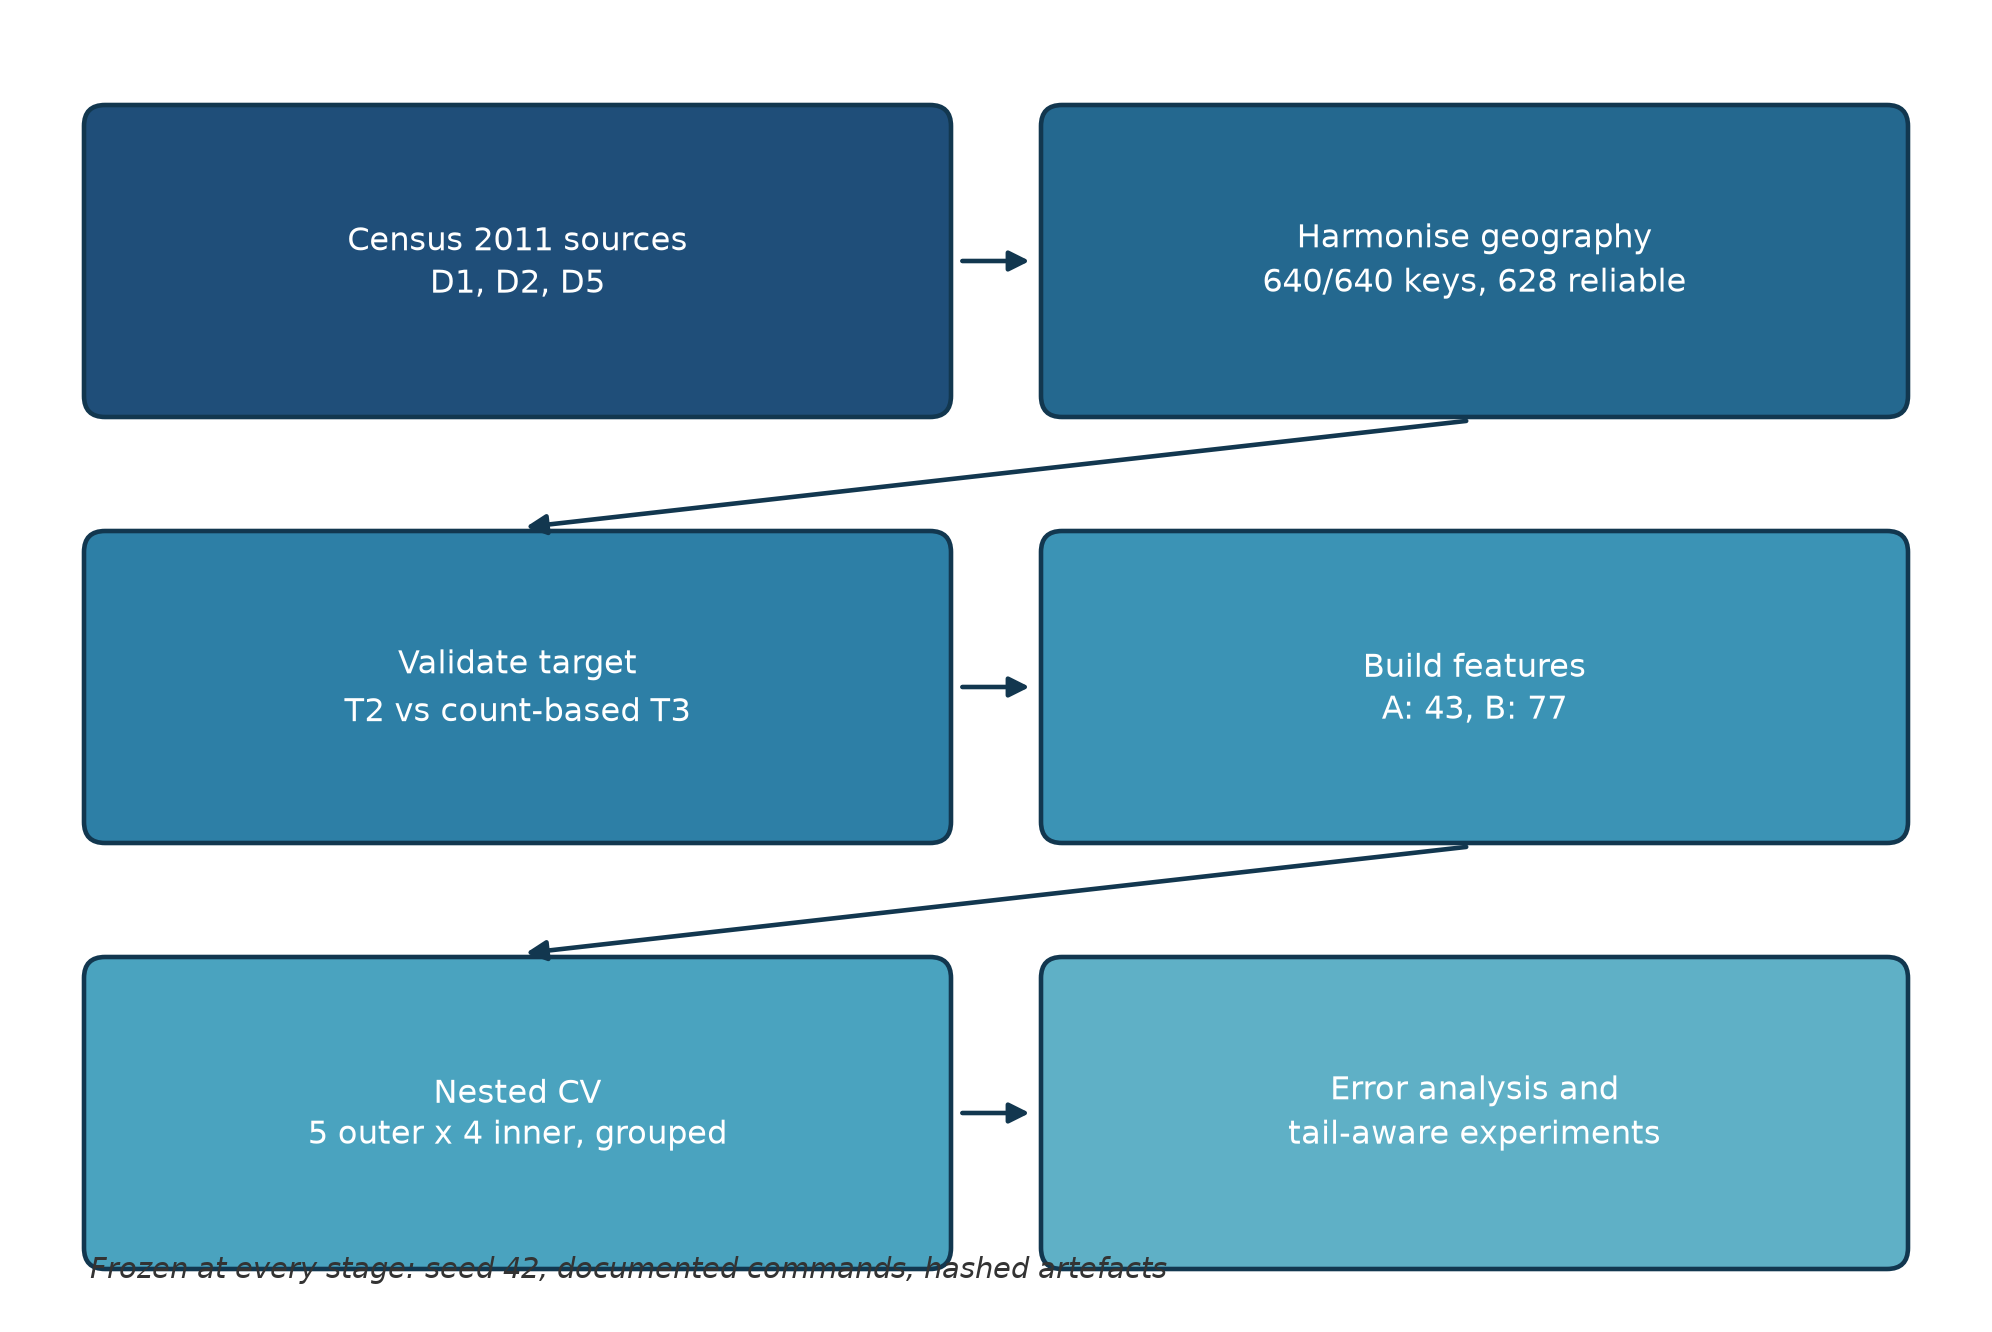
\includegraphics[width=\columnwidth]{fig1_pipeline.png}
\caption{End-to-end workflow. Each stage is a script with a fixed seed and a hashed output, so the reported numbers regenerate from the raw census files.}
\label{fig:pipeline}
\end{figure}

\section{Results and Discussion}

Table III reports the grouped nested cross-validation results. Every family except the single decision tree improves on the mean baseline (MAE 2.4495), and the ordering is consistent with the structure of the problem: penalised linear models and kernel regression lead, while a lone tree is worse than predicting the mean because its piecewise-constant fit does not transfer across states.

\begin{table}[t]
\centering
\caption{Grouped nested cross-validation, fold means. MAE and RMSE in percentage points.}
\label{tab:5998}
\small
\setlength{\tabcolsep}{4pt}
\begin{tabular}{lcccc}
\toprule
\textbf{Configuration / model} & \textbf{MAE} & \textbf{RMSE} & \textbf{R2} & \textbf{Spearman} \\
\midrule
A (640), SVR-RBF & 2.0293 & 2.6144 & 0.1699 & 0.4626 \\
A (640), Ridge & 2.1877 & 2.7957 & 0.0715 & 0.4484 \\
A (628), Extra Trees & 2.0888 & 2.6540 & 0.1837 & 0.4966 \\
B (628), SVR-RBF & 1.7248 & 2.2556 & 0.3992 & 0.6258 \\
B (628), Ridge & 1.7490 & 2.2703 & 0.3992 & 0.6311 \\
B (628), Elastic Net & 1.7476 & 2.2946 & 0.3923 & 0.6444 \\
B (628), mean baseline & 2.4495 & 3.1438 & -0.1157 & - \\
\bottomrule
\end{tabular}
\end{table}

The random-split protocol tells a different story. The best models reach MAE 1.3257 (A, 640), 1.3390 (A, 628) and 1.1401 (B, 628), against grouped values of 2.0293, 2.0888 and 1.7248. The gap of 0.58 to 0.75 percentage points is not a modelling artefact but the quantity of information that districts of the same state share, and it is the reason random splitting is reported only as a reference [12], [13].

\textbf{Configuration A versus B.} On the identical 628 districts and identical folds, Configuration B improved eight of ten families and improved on all five outer folds for seven of them. Support vector regression moved from MAE 2.1714 to 1.7248, Ridge from 2.1845 to 1.7490 and Elastic Net from 2.1963 to 1.7476. The consistency across families and folds supports the value of the additional valid household features; it does not establish a causal role for any of them, since the added variables are correlates of the same underlying development gradient.

\textbf{Model roles.} SVR-RBF achieves the lowest grouped MAE in Configuration B (1.7248) and is reported as the accuracy benchmark. Ridge regression with $\alpha$ = 100 is retained as the primary interpretable model at MAE 1.7490, and Elastic Net as the secondary interpretable model at 1.7476. The 0.0242 percentage-point difference between SVR and Ridge is smaller than the fold-to-fold standard deviation and is not treated as evidence of superiority; the benchmark is not the selected model, and the distinction is maintained throughout.

\textbf{Interpretation.} Ridge selected $\alpha$ = 100 in all five outer folds. Fifty-four of the 77 coefficients preserve their sign across all five folds, with a median standard-deviation to absolute-mean ratio of 0.55; the remainder flip sign and are not interpreted individually. The largest stable coefficients are television share (-0.473), two-person-household share (-0.449), electricity share (-0.394) and radio share (-0.360), with positive coefficients for three-person-household share (+0.313) and non-standard cooking fuel (+0.301). Held-out permutation importance for the benchmark agrees on the dominant block: television share 0.0836, mobile-only share 0.0527, tap-water share 0.0434, telephone share 0.0385 and two-wheeler share 0.0384, with the ten most important features carrying 57\% of total importance. These are predictive associations among correlated indicators measured on a common base, not causal effects, and features whose importance is unstable are reported as such.

\textbf{Error structure.} The aggregate error conceals a systematic pattern. Splitting the out-of-fold predictions by observed outcome, the model is almost unbiased overall (+0.092 percentage points) while under-predicting the 35 districts at or above the 95th percentile (11.20) by 4.510 percentage points, with a tail MAE of 4.527. Individual failures are large: Dhubri is predicted at 7.40 against an observed 17.0, Barpeta at 8.30 against 17.7, Purba Medinipur at 8.04 against 17.2, Murshidabad at 7.04 against 16.0 and Darrang at 8.53 against 17.2. The largest errors concentrate in Assam and West Bengal, where 24 of the 35 extreme districts lie. Approximately 97\% of the tail is under-predicted. This is the compression expected of any variance-reducing estimator, and it is the failure that motivates Section VI.

\section{Tail-Aware Experiments}

The baseline for these experiments is the ratified Ridge model in Configuration B, reused without refitting (arm E0): overall MAE 1.750, p90 MAE 3.648, p95 bias +4.510. Five remedies were registered before execution. E1, E2 and E3 apply sample weights that boost districts above a training-set quantile, with weight increments and thresholds chosen to span mild and aggressive emphasis; E4a and E4b fit linear conditional quantile regressions at $\tau$ = 0.75 and $\tau$ = 0.90 respectively. Selection remained nested: the weights and thresholds of E1-E3 are recomputed inside each training partition and never use validation or test labels, and the outer folds are the frozen Phase 3 folds, so no comparison is contaminated by a fold change.

\begin{table}[t]
\centering
\caption{Tail-aware arms. MAE and bias in percentage points; coverage is empirical at the arm's tau.}
\label{tab:3503}
\small
\setlength{\tabcolsep}{4pt}
\begin{tabular}{lcccccc}
\toprule
\textbf{Arm} & \textbf{MAE} & \textbf{R2} & \textbf{p90 MAE} & \textbf{p95 bias} & \textbf{Sens.} & \textbf{Prec.} \\
\midrule
E0 & 1.750 & 0.468 & 3.648 & +4.510 & 0.371 & 0.520 \\
E1 & 1.915 & 0.398 & 3.032 & +3.693 & 0.543 & 0.388 \\
E2 & 1.975 & 0.350 & 2.831 & +3.435 & 0.686 & 0.387 \\
E3 & 1.985 & 0.347 & 2.807 & +3.271 & 0.600 & 0.300 \\
E4a & 1.914 & 0.375 & 2.624 & +3.109 & 0.629 & 0.324 \\
E4b & 2.912 & -0.302 & 2.331 & +2.994 & 0.543 & 0.170 \\
\bottomrule
\end{tabular}
\end{table}

Every arm reduced tail error and tail bias, and every arm paid for it (Table IV). The weighted arms cut the p95 bias by 18.1\% to 27.5\% while raising overall MAE by 9.5\% to 13.5\%; the quantile arms cut it by 31.1\% and 33.6\% while raising MAE by 9.4\% and 66.4\%. The implied exchange rate is roughly 0.12 to 0.21 percentage points of overall MAE per percentage point of tail bias recovered, so eliminating the 4.5-point tail bias entirely would cost of the order of half a point of overall MAE.

The arms also illustrate two distinct failure modes. E4b over-corrects: it improves Assam substantially while making West Bengal worse, with 63\% of its tail-error reduction concentrated in a single state. And all five arms lose precision at the frozen p90 threshold: sensitivity rises to 0.54-0.69 but precision falls to 0.17-0.39, because flagging more districts necessarily flags more false positives.

Six acceptance criteria were registered in advance. C1 required a 30\% reduction in tail bias together with an improvement in p90 MAE; the weighted arms met the p90 condition but reached only 18-28\% on bias, and for the quantile arms C1 and C2 are not applicable because a conditional quantile is not a mean predictor. C2 capped the overall cost at 5\%; every arm exceeded it. C3 required improvement in at least three of the four folds containing tail districts, which E1-E4a met. C4 required the gain to be spread across states, which E4b failed. C5, guarding against over-correction, passed everywhere. C6 required precision of at least 0.40, which every arm failed. No challenger satisfied the criteria and no model was promoted; Ridge remains the primary model.

Uncertainty was assessed with a paired bootstrap [19] over 2,000 resamples. For E1 the change in MAE relative to E0 was +0.165 with a 95\% interval of [+0.022, +0.327], and the change in tail bias was -0.817 with interval [-1.077, -0.487]; both exclude zero, so the trade-off is real rather than noise. Quantile calibration was weaker than the nominal level: E4a achieved empirical coverage of 0.670 at $\tau$ = 0.75 and E4b 0.825 at $\tau$ = 0.90, both below target, so better pinball loss did not translate into calibrated conditional quantiles [14], [15]. Subgroup coverage at the extreme threshold rests on 35 districts and is reported descriptively.

The registered conclusion is therefore negative and is quoted without embellishment: “No improvement was demonstrated using the tested tail-aware approaches. Limited predictor information is one possible explanation, but cannot be established from these experiments alone. Further evidence, potentially including additional independent predictors, would be required to establish an information ceiling.” The experiments bound the trade-off and rule out this class of remedy; they do not establish that the tail gap is intrinsic to the predictor set.

\section{Limitations}

The study is historical: it describes 2011 conditions in the 2011 administrative geography, and no claim about present-day housing is made or supported. The design is ecological, so district aggregates cannot identify household-level risk, and the results are subject to the ecological fallacy if read that way [20]. No causal interpretation is available from a cross-sectional observational design of this kind.

Explanatory power is modest. An $R^2$ of 0.3992 leaves roughly 60\% of between-district variance unexplained, so the model ranks districts reasonably but forecasts magnitudes only coarsely. Twelve districts are unscorable in the expanded configuration, and their exclusion is not random with respect to state. The tail is small and geographically concentrated, so tail conclusions are correspondingly fragile, and the number of state-grouped outer folds is five, which limits the precision of any fold-level claim. As noted in Section IV, the Phase 2 feature screen was computed on the full sample, so the feature set is not fully nested and a small optimistic bias cannot be excluded. Finally, no contemporary validation data exists, so the temporal stability of the relationship is untested.

\section{Conclusion and Future Work}

A district-level predictive benchmark for dilapidated-house prevalence was constructed from Census 2011 data, with the target definition validated against an independent count-based reconstruction (r = 0.9994) before any modelling. Under nested state-grouped cross-validation, expanding the feature set with household-normalised housing variables improved eight of ten model families, and support vector regression achieved the lowest error (MAE 1.7248, $R^2$ 0.3992, Spearman 0.6258). Ridge regression at $\alpha$ = 100, with 54 of 77 coefficients sign-stable across folds, was retained as the primary interpretable model at MAE 1.7490. Random cross-validation understated error by 0.58 to 0.75 percentage points, confirming that geographic grouping is essential rather than cosmetic.

The study's most informative result is negative. The selected model under-predicts the most deprived districts by 4.510 percentage points while remaining nearly unbiased overall, and five pre-registered remedies that reduced this bias by up to a third all failed their cost, state-consistency or precision criteria. Within the predictors available, the tail gap appears to be purchased down only at a disproportionate cost in overall accuracy. Future work should therefore add independent information rather than additional loss functions: housing age and construction material, climate exposure, migration, and updated census rounds. Spatially explicit validation and per-district prediction intervals are the natural methodological extensions, and none of them has been attempted here.

\section*{References}
\small
\begin{thebibliography}{99}
\bibitem{ref} Office of the Registrar General and Census Commissioner, India, “Houselisting and Housing Census, 2011: housing condition and amenities tables,” Ministry of Home Affairs, New Delhi, 2011. [Online]. Available: https://censusindia.gov.in
\bibitem{ref} Office of the Registrar General and Census Commissioner, India, “Primary Census Abstract, Census of India 2011,” Ministry of Home Affairs, New Delhi, 2011. [Online]. Available: https://censusindia.gov.in
\bibitem{ref} United Nations Human Settlements Programme, The Challenge of Slums: Global Report on Human Settlements 2003. London, U.K.: Earthscan, 2003.
\bibitem{ref} A. E. Hoerl and R. W. Kennard, “Ridge regression: biased estimation for nonorthogonal problems,” Technometrics, vol. 12, no. 1, pp. 55–67, 1970, doi: 10.1080/00401706.1970.10488634.
\bibitem{ref} R. Tibshirani, “Regression shrinkage and selection via the lasso,” Journal of the Royal Statistical Society: Series B, vol. 58, no. 1, pp. 267–288, 1996, doi: 10.1111/j.2517-6161.1996.tb02080.x.
\bibitem{ref} H. Zou and T. Hastie, “Regularization and variable selection via the elastic net,” Journal of the Royal Statistical Society: Series B, vol. 67, no. 2, pp. 301–320, 2005, doi: 10.1111/j.1467-9868.2005.00503.x.
\bibitem{ref} L. Breiman, “Random forests,” Machine Learning, vol. 45, no. 1, pp. 5–32, 2001, doi: 10.1023/A:1010933404324.
\bibitem{ref} J. H. Friedman, “Greedy function approximation: a gradient boosting machine,” Annals of Statistics, vol. 29, no. 5, pp. 1189–1232, 2001, doi: 10.1214/aos/1013203451.
\bibitem{ref} P. Geurts, D. Ernst, and L. Wehenkel, “Extremely randomized trees,” Machine Learning, vol. 63, no. 1, pp. 3–42, 2006, doi: 10.1007/s10994-006-6226-1.
\bibitem{ref} C. Cortes and V. Vapnik, “Support-vector networks,” Machine Learning, vol. 20, no. 3, pp. 273–297, 1995, doi: 10.1007/BF00994018.
\bibitem{ref} T. M. Cover and P. E. Hart, “Nearest neighbor pattern classification,” IEEE Transactions on Information Theory, vol. 13, no. 1, pp. 21–27, 1967, doi: 10.1109/TIT.1967.1053964.
\bibitem{ref} D. R. Roberts et al., “Cross-validation strategies for data with temporal, spatial, hierarchical, or phylogenetic structure,” Ecography, vol. 40, no. 8, pp. 913–929, 2017, doi: 10.1111/ecog.02881.
\bibitem{ref} P. Ploton et al., “Spatial validation reveals poor predictive performance of large-scale ecological mapping models,” Nature Communications, vol. 11, art. 4540, 2020, doi: 10.1038/s41467-020-18321-y.
\bibitem{ref} R. Koenker and G. Bassett, “Regression quantiles,” Econometrica, vol. 46, no. 1, pp. 33–50, 1978, doi: 10.2307/1913643.
\bibitem{ref} E. B. Wilson, “Probable inference, the law of succession, and statistical inference,” Journal of the American Statistical Association, vol. 22, no. 158, pp. 209–212, 1927, doi: 10.1080/01621459.1927.10502953.
\bibitem{ref} L. D. Brown, T. T. Cai, and A. DasGupta, “Interval estimation for a binomial proportion,” Statistical Science, vol. 16, no. 2, pp. 101–133, 2001, doi: 10.1214/ss/1009213286.
\bibitem{ref} F. Pedregosa et al., “Scikit-learn: machine learning in Python,” Journal of Machine Learning Research, vol. 12, pp. 2825–2830, 2011. [Online]. Available: https://jmlr.org/papers/v12/pedregosa11a.html
\bibitem{ref} R. J. Hyndman and A. B. Koehler, “Another look at measures of forecast accuracy,” International Journal of Forecasting, vol. 22, no. 4, pp. 679–688, 2006, doi: 10.1016/j.ijforecast.2006.03.001.
\bibitem{ref} B. Efron and R. J. Tibshirani, An Introduction to the Bootstrap. New York, NY, USA: Chapman \& Hall, 1993.
\bibitem{ref} W. S. Robinson, “Ecological correlations and the behavior of individuals,” American Sociological Review, vol. 15, no. 3, pp. 351–357, 1950, doi: 10.2307/2087176.
\end{thebibliography}

\end{document}
